
\section{Biological background}

\begin{frame}
\frametitle{Coral Reef}
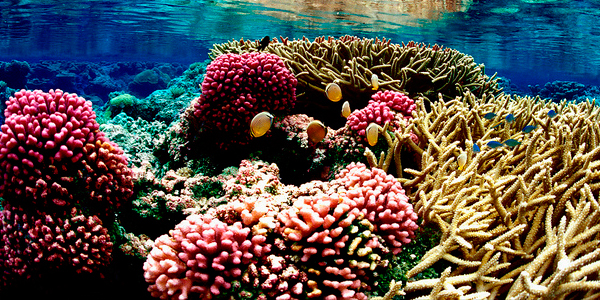
\includegraphics[scale=.175]{./US-Wildlife-coral-1.jpg}
\begin{itemize}
\item A complex aquatic ecosystem physically supported by calcium carbonate secretions of the colorful stone coral. \\
\item Modeling approach by Li-Wang-Zhang-Hastings is to describe the relationships between macroalgae, algal turfs, and corals (Li et al., 2014).
\end{itemize}
\end{frame}

\begin{frame}
\frametitle{Positives}
\begin{itemize}
\item Naturally filter the water by reducing the levels of phosphate and nitrogenous waste.
\item Provide hiding places for fishes and invertebrates.
\item Get their energy from the sun and convert it into food for the rest of the reef food web. 
\end{itemize}
\end{frame}

\begin{frame}
\frametitle{Coral Reef Ecosystem} 

McClanahan identifies three major components:
\begin{itemize}
\item Primary producers (coral and algae)\\
\item Herbivores (e.g. parrotfish)\\
\item Carnivores (McClanahan, 1994).
\end{itemize}
\end{frame}

\begin{frame}
\frametitle{Reef Food Web}
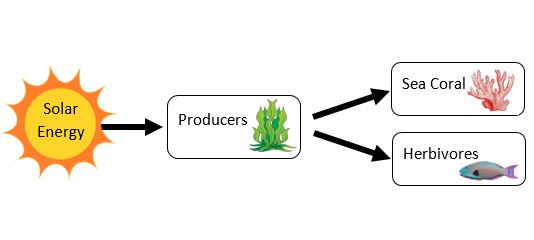
\includegraphics[scale=.8]{./CoralFoodWeb}
\end{frame}

\begin{frame}
\frametitle{Negatives}
\begin{itemize}
\item At low grazing levels, the macroalgal population increases and competes with the coral population for space.
\item This competition alters the microbial communities associated with corals increasing pathogens on corals.
\item Macroalgal abundance may lead to reef degradation.
\item Coral mortality is generally followed by algal recruitment.
\end{itemize}
\end{frame}

\begin{frame}
\frametitle{Coral Reef Dynamics}
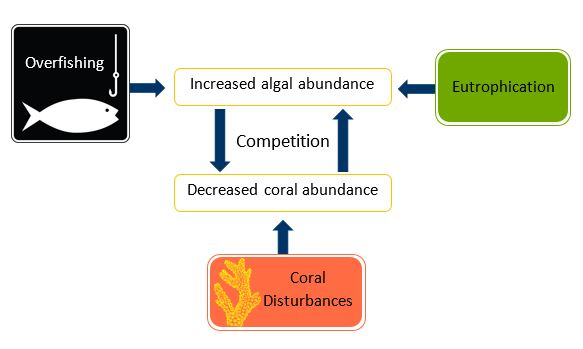
\includegraphics[scale=.7]{./CoralDynamics}
\end{frame}

\begin{frame}
\frametitle{Coral Reef Dynamics}
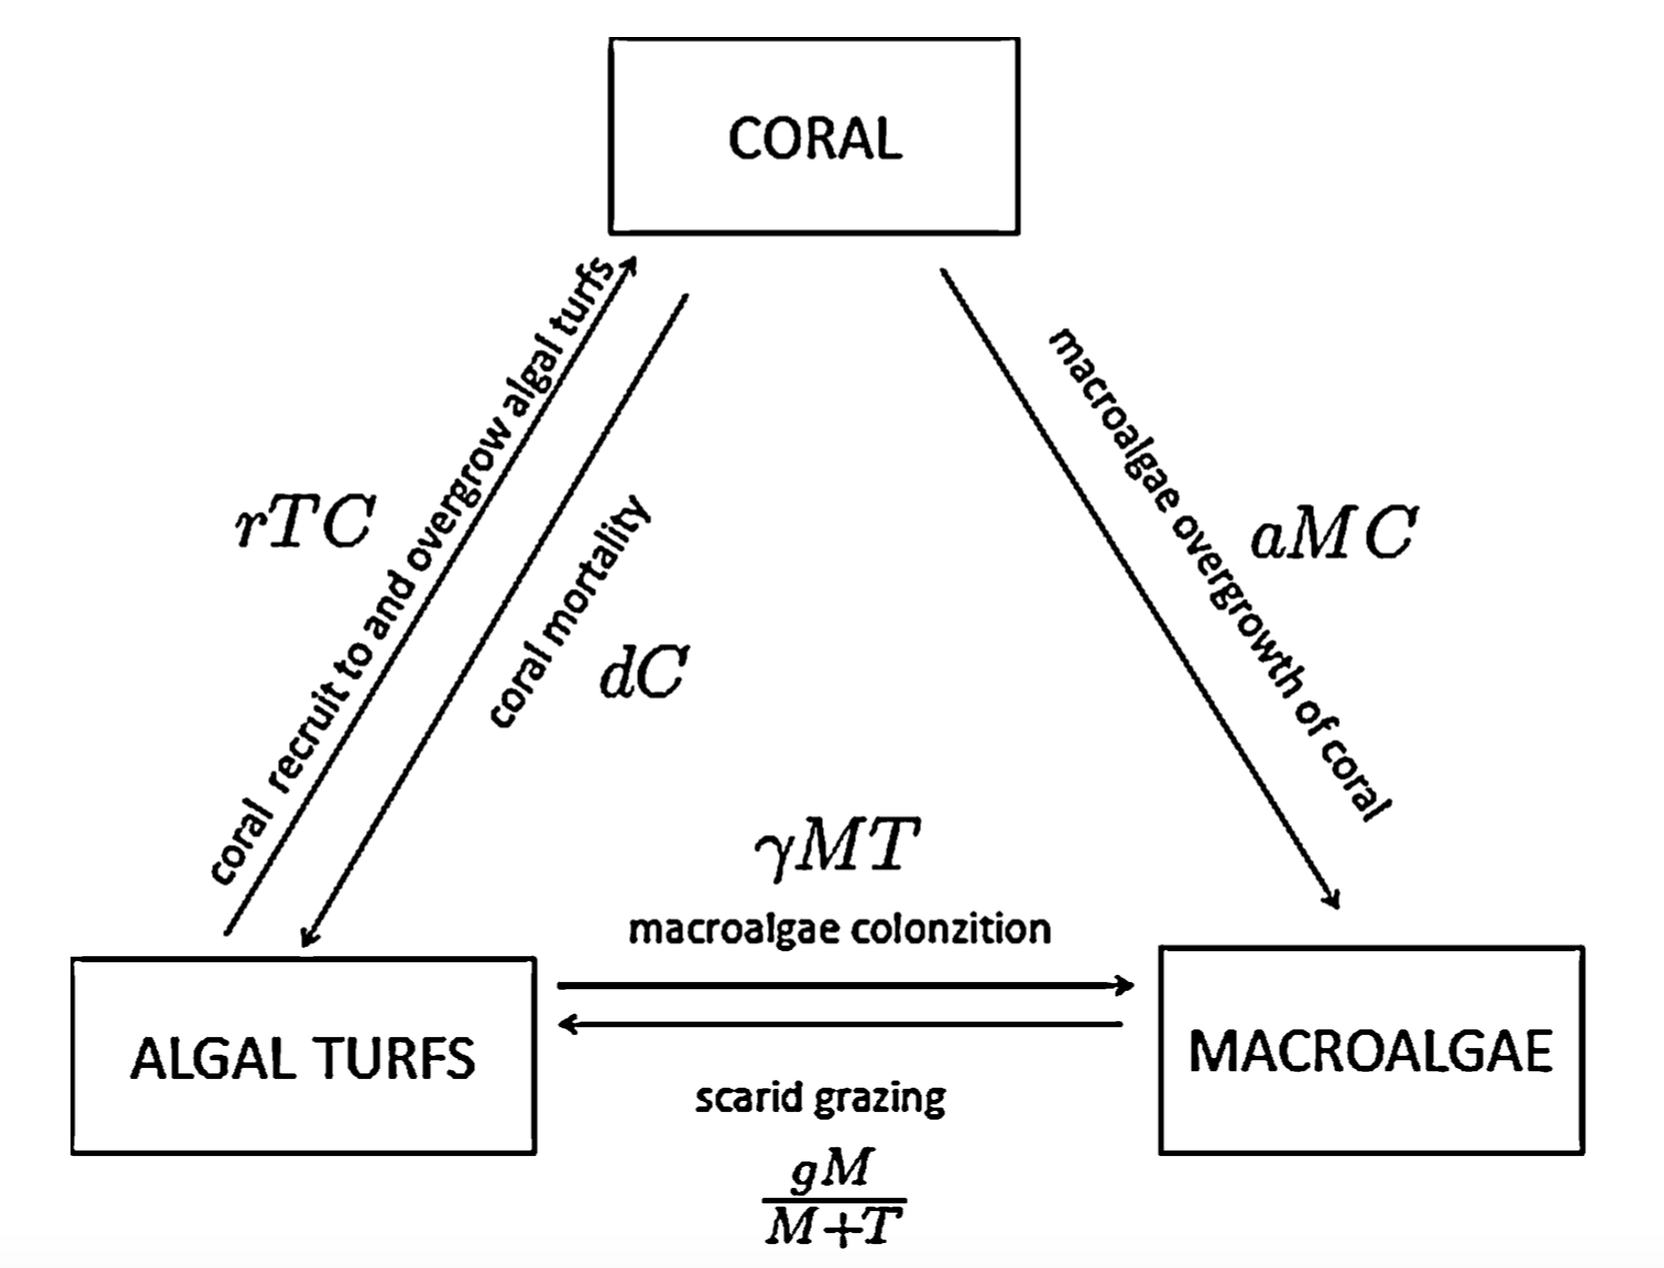
\includegraphics[scale=.175]{./coral-reef-triangle.png}
\end{frame}

%%% Local Variables:
%%% mode: latex
%%% TeX-master: "Presentation2"
%%% End:
